\documentclass[a4paper,14pt]{extarticle}

\usepackage[T2A]{fontenc}
\usepackage[utf8]{inputenc}
\usepackage[russian]{babel}

\usepackage{extsizes}

\usepackage{setspace}
\onehalfspacing

\usepackage{amsmath, amssymb}

\usepackage{graphicx}
\usepackage{float}

\usepackage{hyperref}

\usepackage{indentfirst}
\setlength{\parindent}{1.25cm}

\usepackage{geometry}
\geometry{
    left=30mm,
    right=15mm,
    top=20mm,
    bottom=20mm
}

\usepackage{booktabs}

\usepackage{listings}
\usepackage{xcolor}

\usepackage{caption}

\usepackage{tocloft}

\usepackage{titlesec}

\titleformat{\section}
  {\bfseries\fontsize{16}{18}\selectfont}
  {\thesection}{1em}{}

\titleformat{\subsection}
  {\bfseries\fontsize{14}{16}\selectfont}
  {\thesubsection}{1em}{}

\renewcommand{\cftsecleader}{\cftdotfill{\cftdotsep}}
\renewcommand{\cftsubsecleader}{\cftdotfill{\cftdotsep}}

\definecolor{codegreen}{rgb}{0,0.6,0}
\definecolor{codegray}{rgb}{0.5,0.5,0.5}
\definecolor{codepurple}{rgb}{0.58,0,0.82}
\definecolor{backcolour}{rgb}{0.95,0.95,0.92}

\lstdefinestyle{mystyle}{
    backgroundcolor=\color{backcolour},
    commentstyle=\color{codegreen},
    keywordstyle=\color{magenta},
    numberstyle=\tiny\color{codegray},
    stringstyle=\color{codepurple},
    basicstyle=\ttfamily\small,
    breaklines=true,
    numbers=left,
    numbersep=5pt,
    language=Python,
    frame=single
}

\lstset{style=mystyle}

\hypersetup{
    colorlinks=true,
    linkcolor=black,
    citecolor=black,
    filecolor=black,
    urlcolor=blue
}
\begin{document}
\begin{titlepage}
\begin{center}
\textsc{Санкт-Петербургский государственный университет\\
Математико-механический факультет\\
Кафедра физической механики\\}

\vfill

\textsc{Методы измерений и электромеханические системы\\[3mm]}
Отчёт по лабораторной работе №1\\[6mm]


\textbf{\large<<Измерение электронным частотомером Ч3-32 периода
следования импульсов>>}

\vfill
\end{center}

\hfill
\begin{minipage}{.5\textwidth}
Выполнил студент:\\[2mm] 
Кручинина Екатерина Васильевна\\
группа: 24.Б51-мм\\[5mm]

Проверил:\\[2mm] 
к.ф.-м.н., доцент\\
Кац Виктор Михайлович
\end{minipage}%
\vfill
\begin{center}
 Санкт-Петербург, 2026 г.
\end{center}
\end{titlepage}


\tableofcontents
\newpage

\section{Введение}

\subsection{Цель работы}
Целью данной лабораторной работы является ознакомление с эксперементальной установкой, измерение электромеханических характеристик, а также получение навыков обработки экспериментальных данных.

\subsection{Решаемые задачи}

В ходе выполнения работы решаются следующие задачи:

\begin{itemize}
\item Изучение принципа действия измерительной установки
\item Проведение серии измерений
\item Статистическая обработка результатов
\item Оценка погрешностей и формулировка выводов
\end{itemize}

\newpage

\section{Основная часть}

\subsection{Теоретическая часть}

Частотометр - прибор, предназначенный для измерения частоты, то есть периода колебаний электрического сигнала за определенный временной интервал. 
Период следования импульсов \(T\) связан с частотой повторения \(f\) соотношением:

\begin{equation}
f = \frac{1}{T}.
\end{equation}

Принцип работы частотометра основан на подсчете числа импульсов за определенный период времени. При измерении периода определяется время между одинаковыми фазовыми состояниями соседних импульсов.


\subsection{Эксперимент}
\textbf{Описание экспериментальной установки:}

В работе проводилось измерение периода следования импульсов, задаваемых на выходе генератора сигналов. От генератора на вход электронного частотомера подавалась последовательность трапецеидальных импульсов, параметры которых задавались преподавателем.

В качестве генератора использовался генератор импульсов Г5-2А, а измерение периода выполнялось электронным частотомером Ч3-32.

Для того чтобы повысить точность определения периода и уменьшить случайную погрешность, измерения проводились на двух шкалах прибора — грубой и точной.


\begin{figure}[H]
\centering
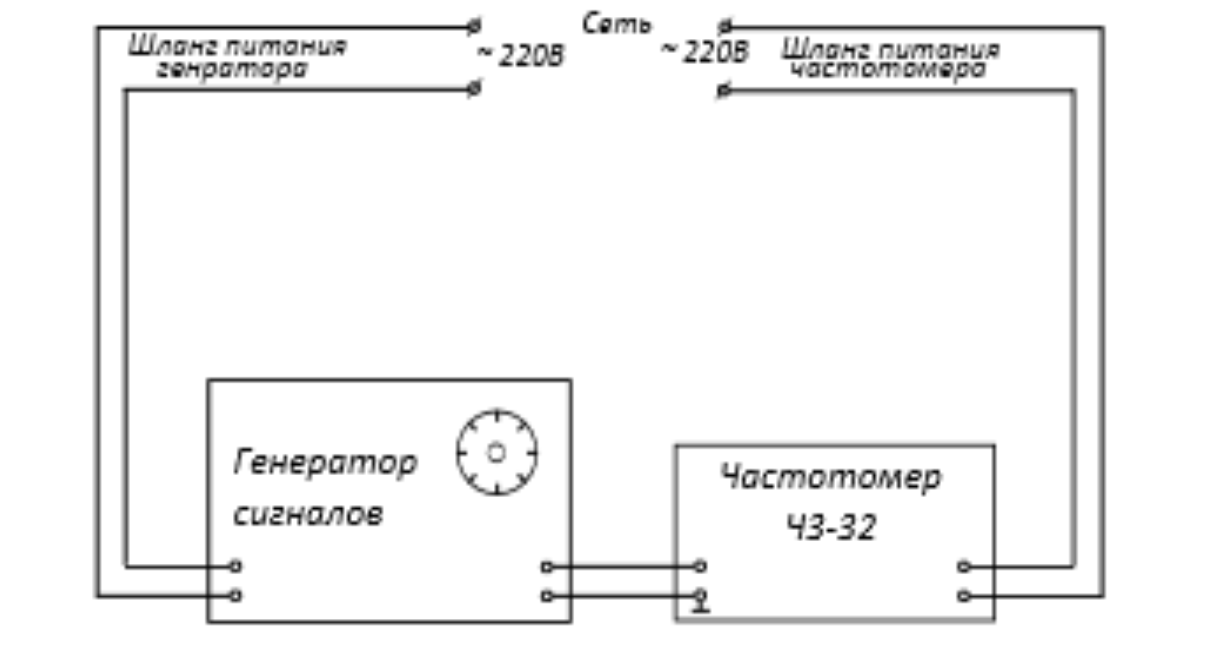
\includegraphics[width=0.8\textwidth]{scheme.png}
\caption{Блок-схема экспериментальной установки}
\end{figure}

\textbf{Эксперимент проводился в следующей последовательности:}

\begin{enumerate}
\item Ознакомление с работой частотомера и выбор шкалы для измерения периода.
\item Измерение периода следования импульсов на грубой шкале прибора (диапазон $10^{-6}$).
\item Переключение шкалы частотометра с грубой на точную.
\item Проведение серии измерений по точной шкале прибора (диапазон $10^{-4}$).
\item Запись результатов измерений в таблицы для последующей обработки.
\end{enumerate}

\subsection{Обработка результатов измерений}

По результатам серии измерений определялось среднее значение периода следования импульсов.

Среднее значение периода вычислялось по формуле:

\begin{equation}
\overline{T} = \frac{1}{n}\sum_{i=1}^{n} T_i,
\end{equation}

где \(T_i\) — результаты отдельных измерений, \(n\) — число измерений.

\begin{equation}
\overline{T} = 273,389,
\end{equation}
среднее значение периода, полученное на основе обработки резултатов полученных с точной шкалы.

Далее все графики и таблицы строятся на основе результатов, полученных с точной шкалы.

Проверялось не изменяется ли измеряемая величина регулярным образом с течением времени. Для этого строился график зависимости результатов наблюдений от времени.

\begin{figure}[H]
\centering
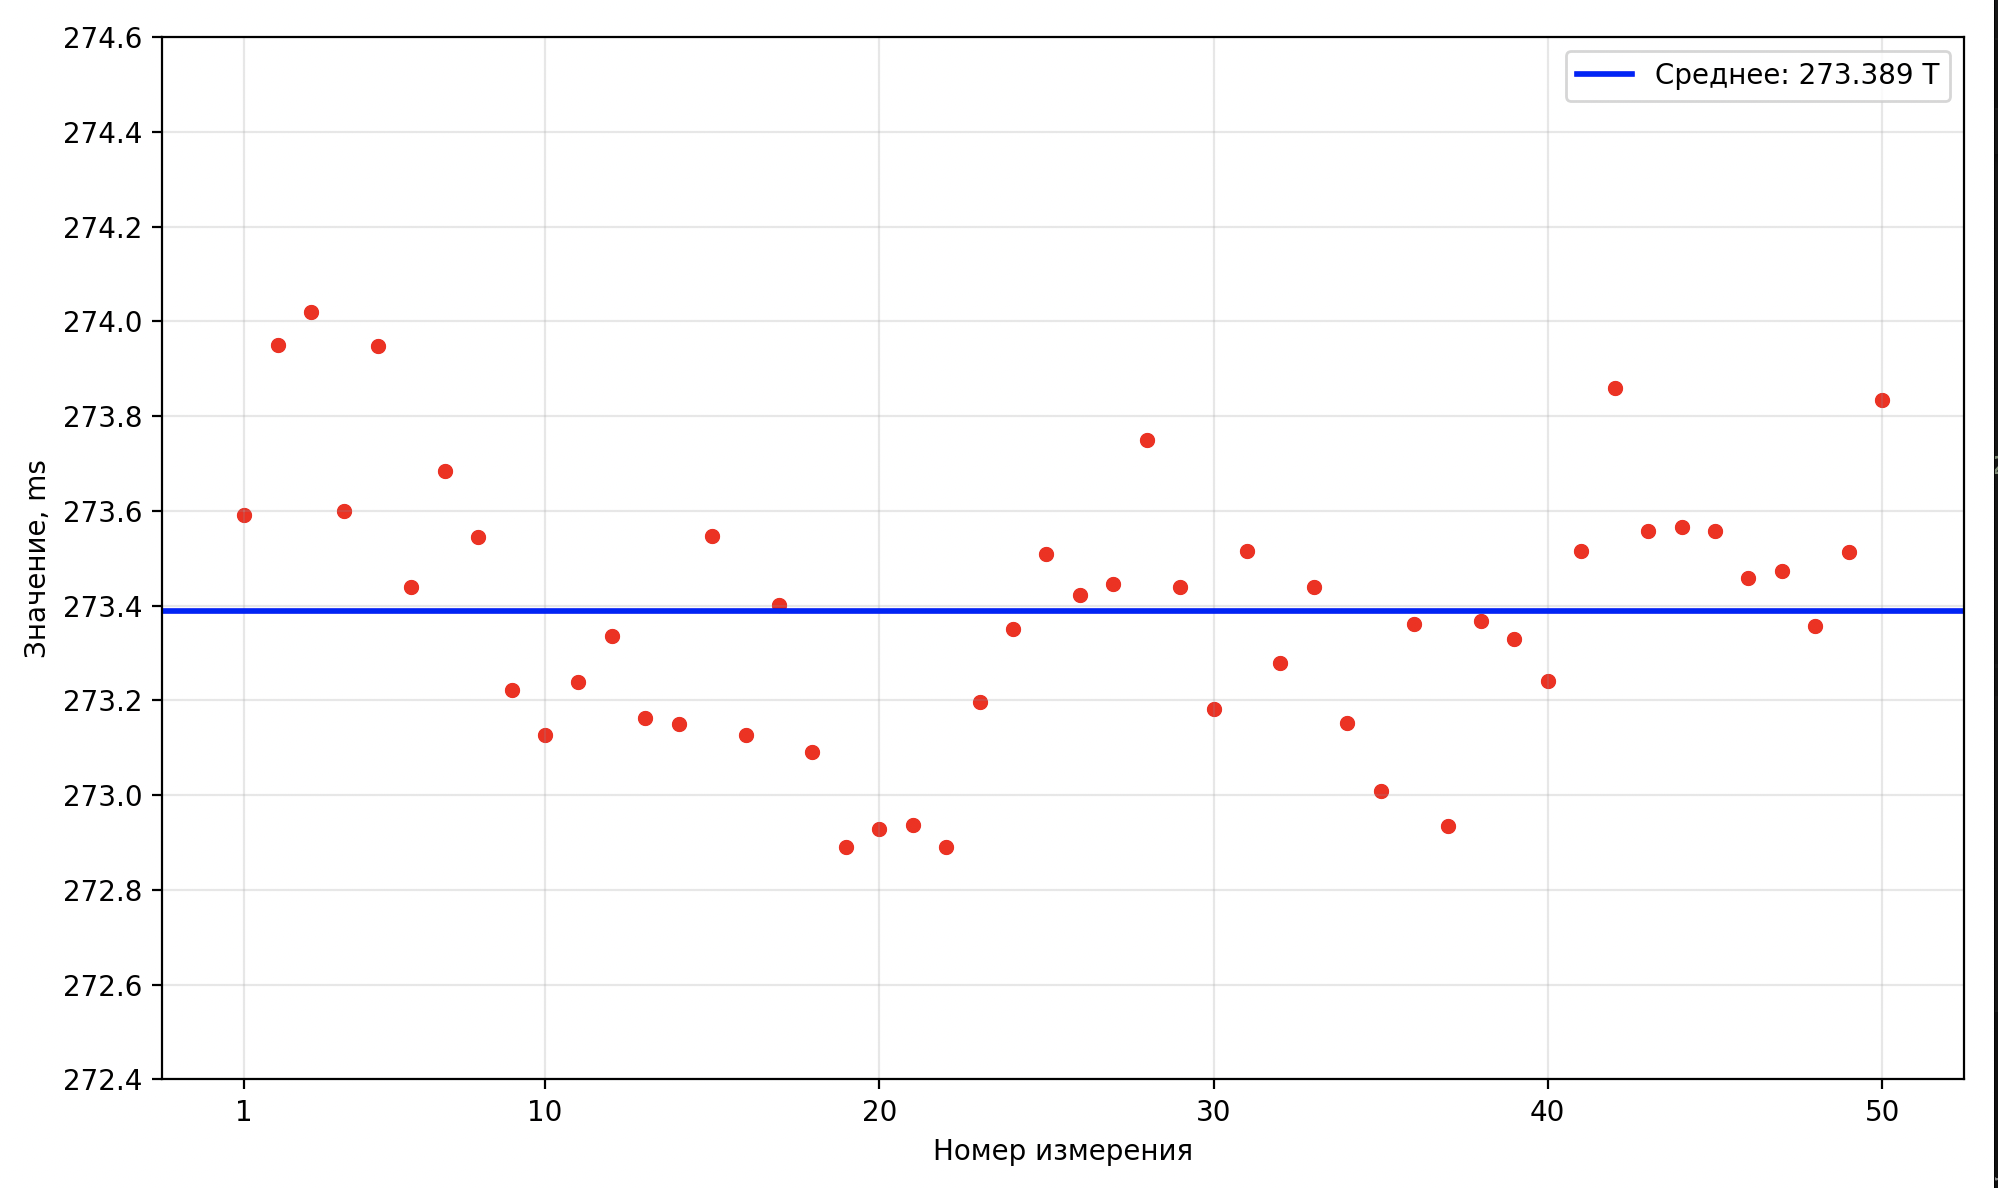
\includegraphics[width=0.8\textwidth]{drift graph.png}
\caption{Зависимость результатов наблюдений от времени}
\end{figure}

На основании построенного графика было установлено, что дрейф отсутствует, следовательно можно переходить к построению гистограммы.

Для начала на числовую ось наносились все результаты отдельных
наблюдений и установливался диапазон, в котором находились все полученные результаты наблюдений.

\begin{figure}[H]
\centering
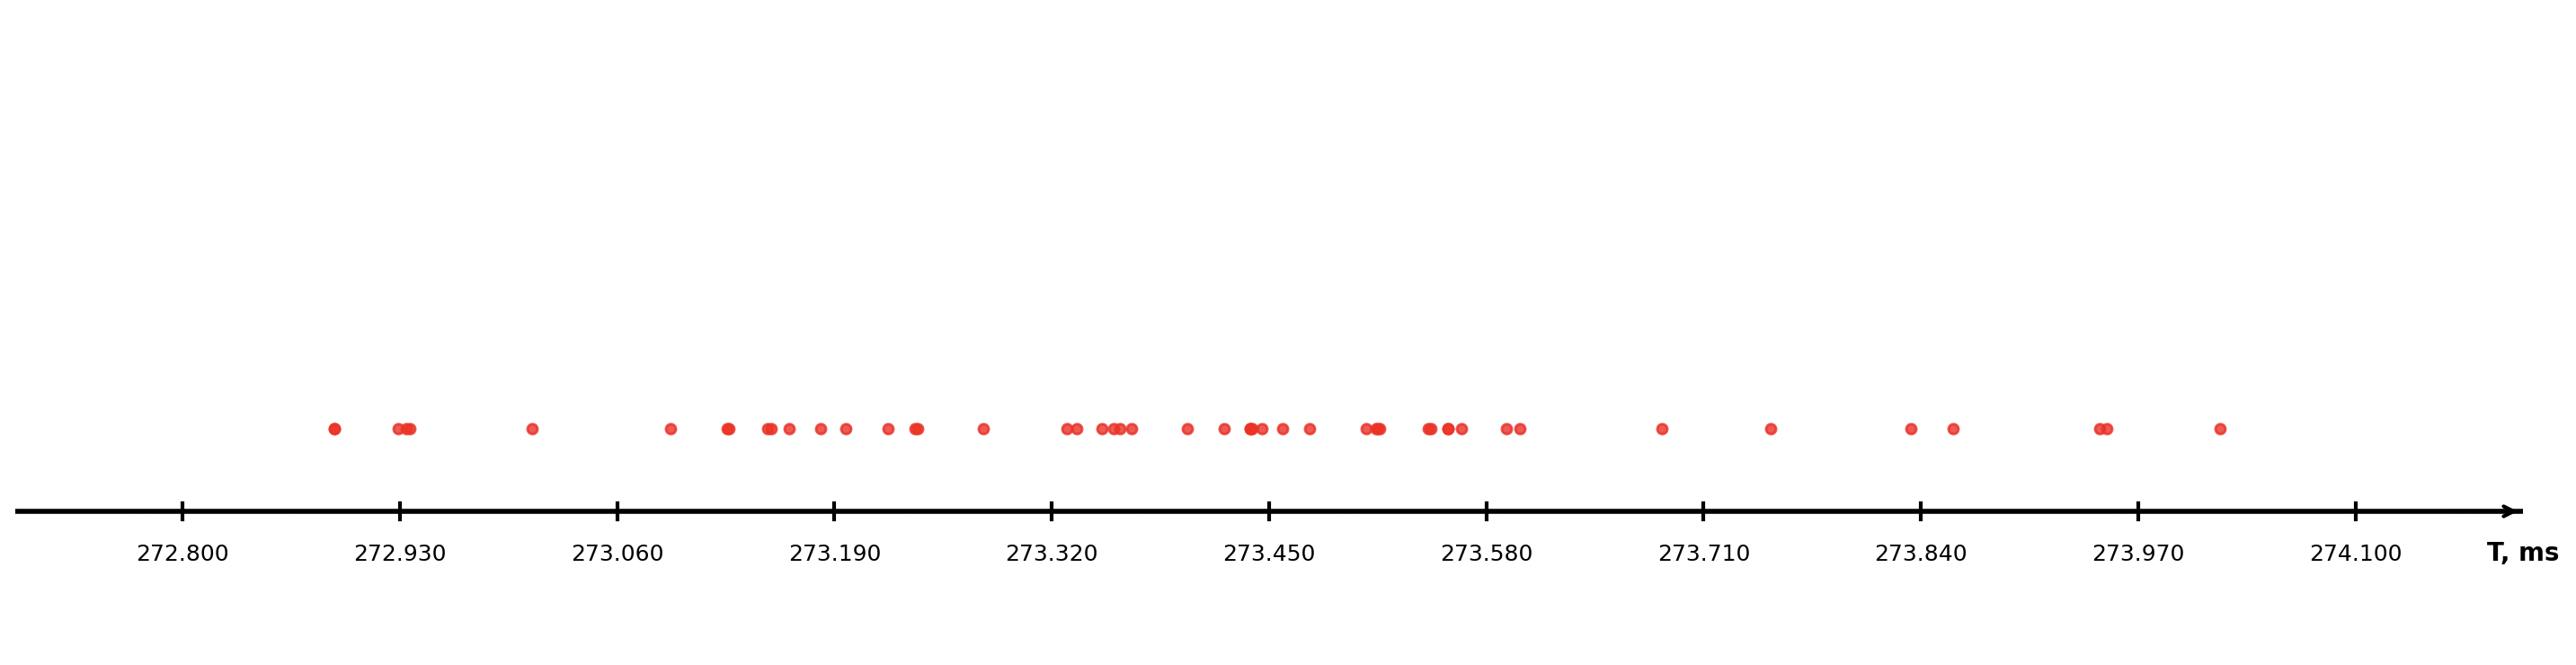
\includegraphics[width=0.8\textwidth]{scatter plot.png}
\caption{Результаты наблюдений на числовой оси}
\end{figure}

Далее были определены Tmin = 272,891 мс и Tmax = 274,019 мс. Диапозон был разбит на 10 интервалов с шагом 0,130 мс.
\begin{figure}[H]
\centering
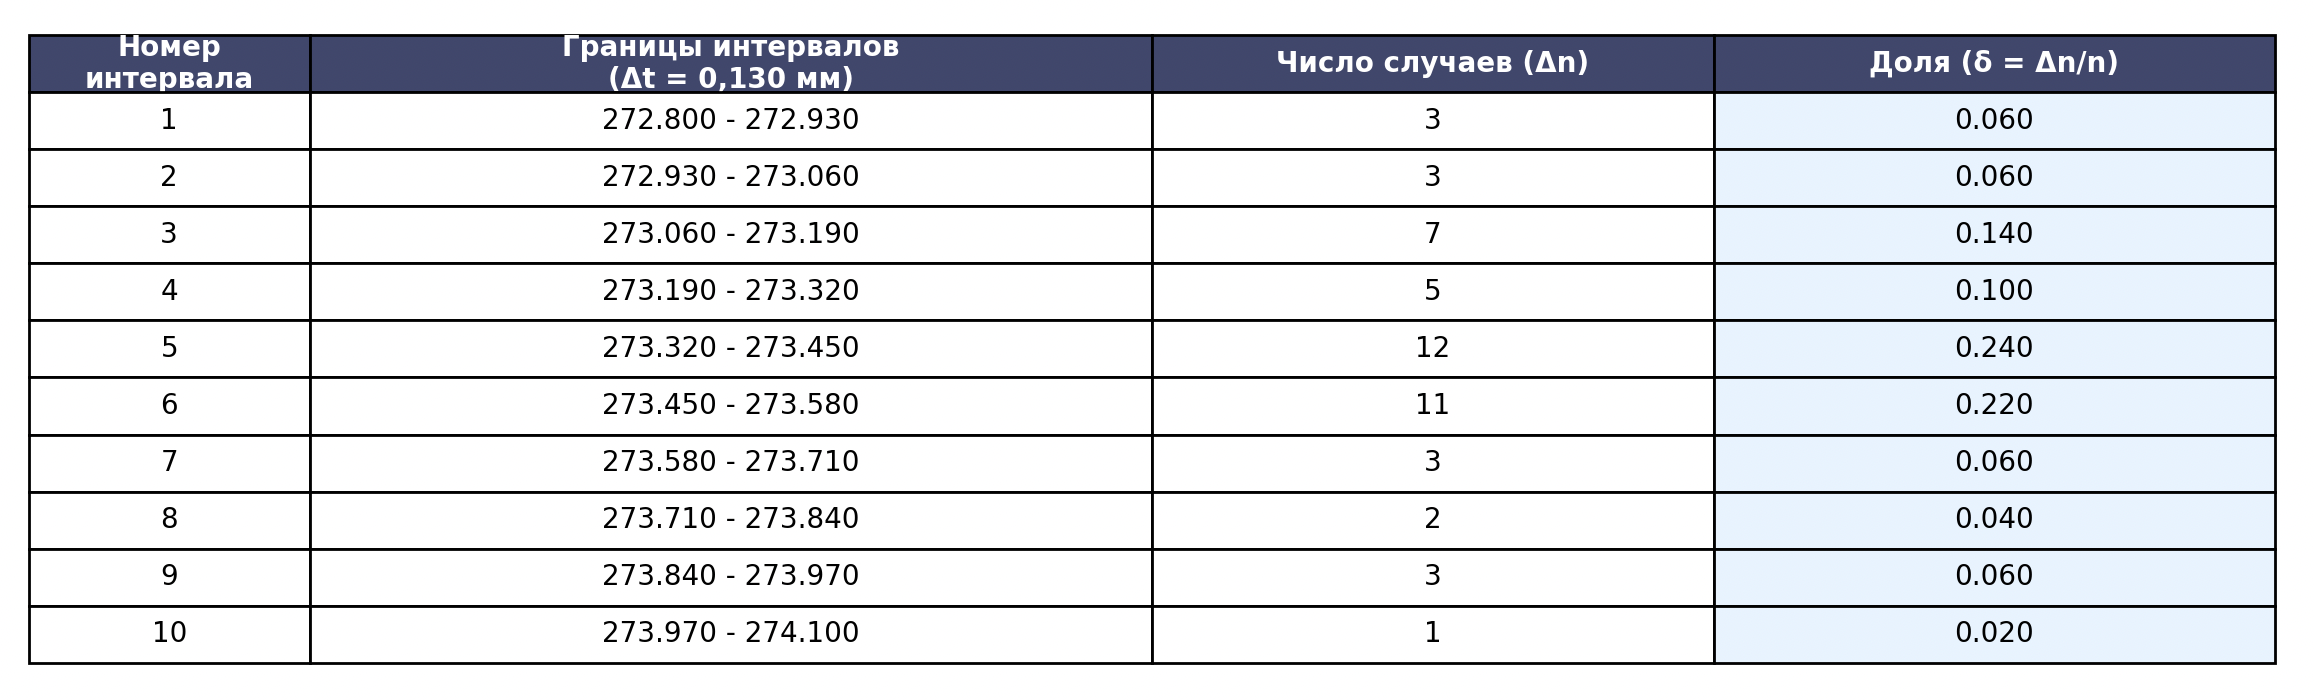
\includegraphics[width=0.8\textwidth]{table.png}
\caption{Таблица 1}
\end{figure}
На основании таблицы строилась гистограмма
\begin{figure}[H]
\centering
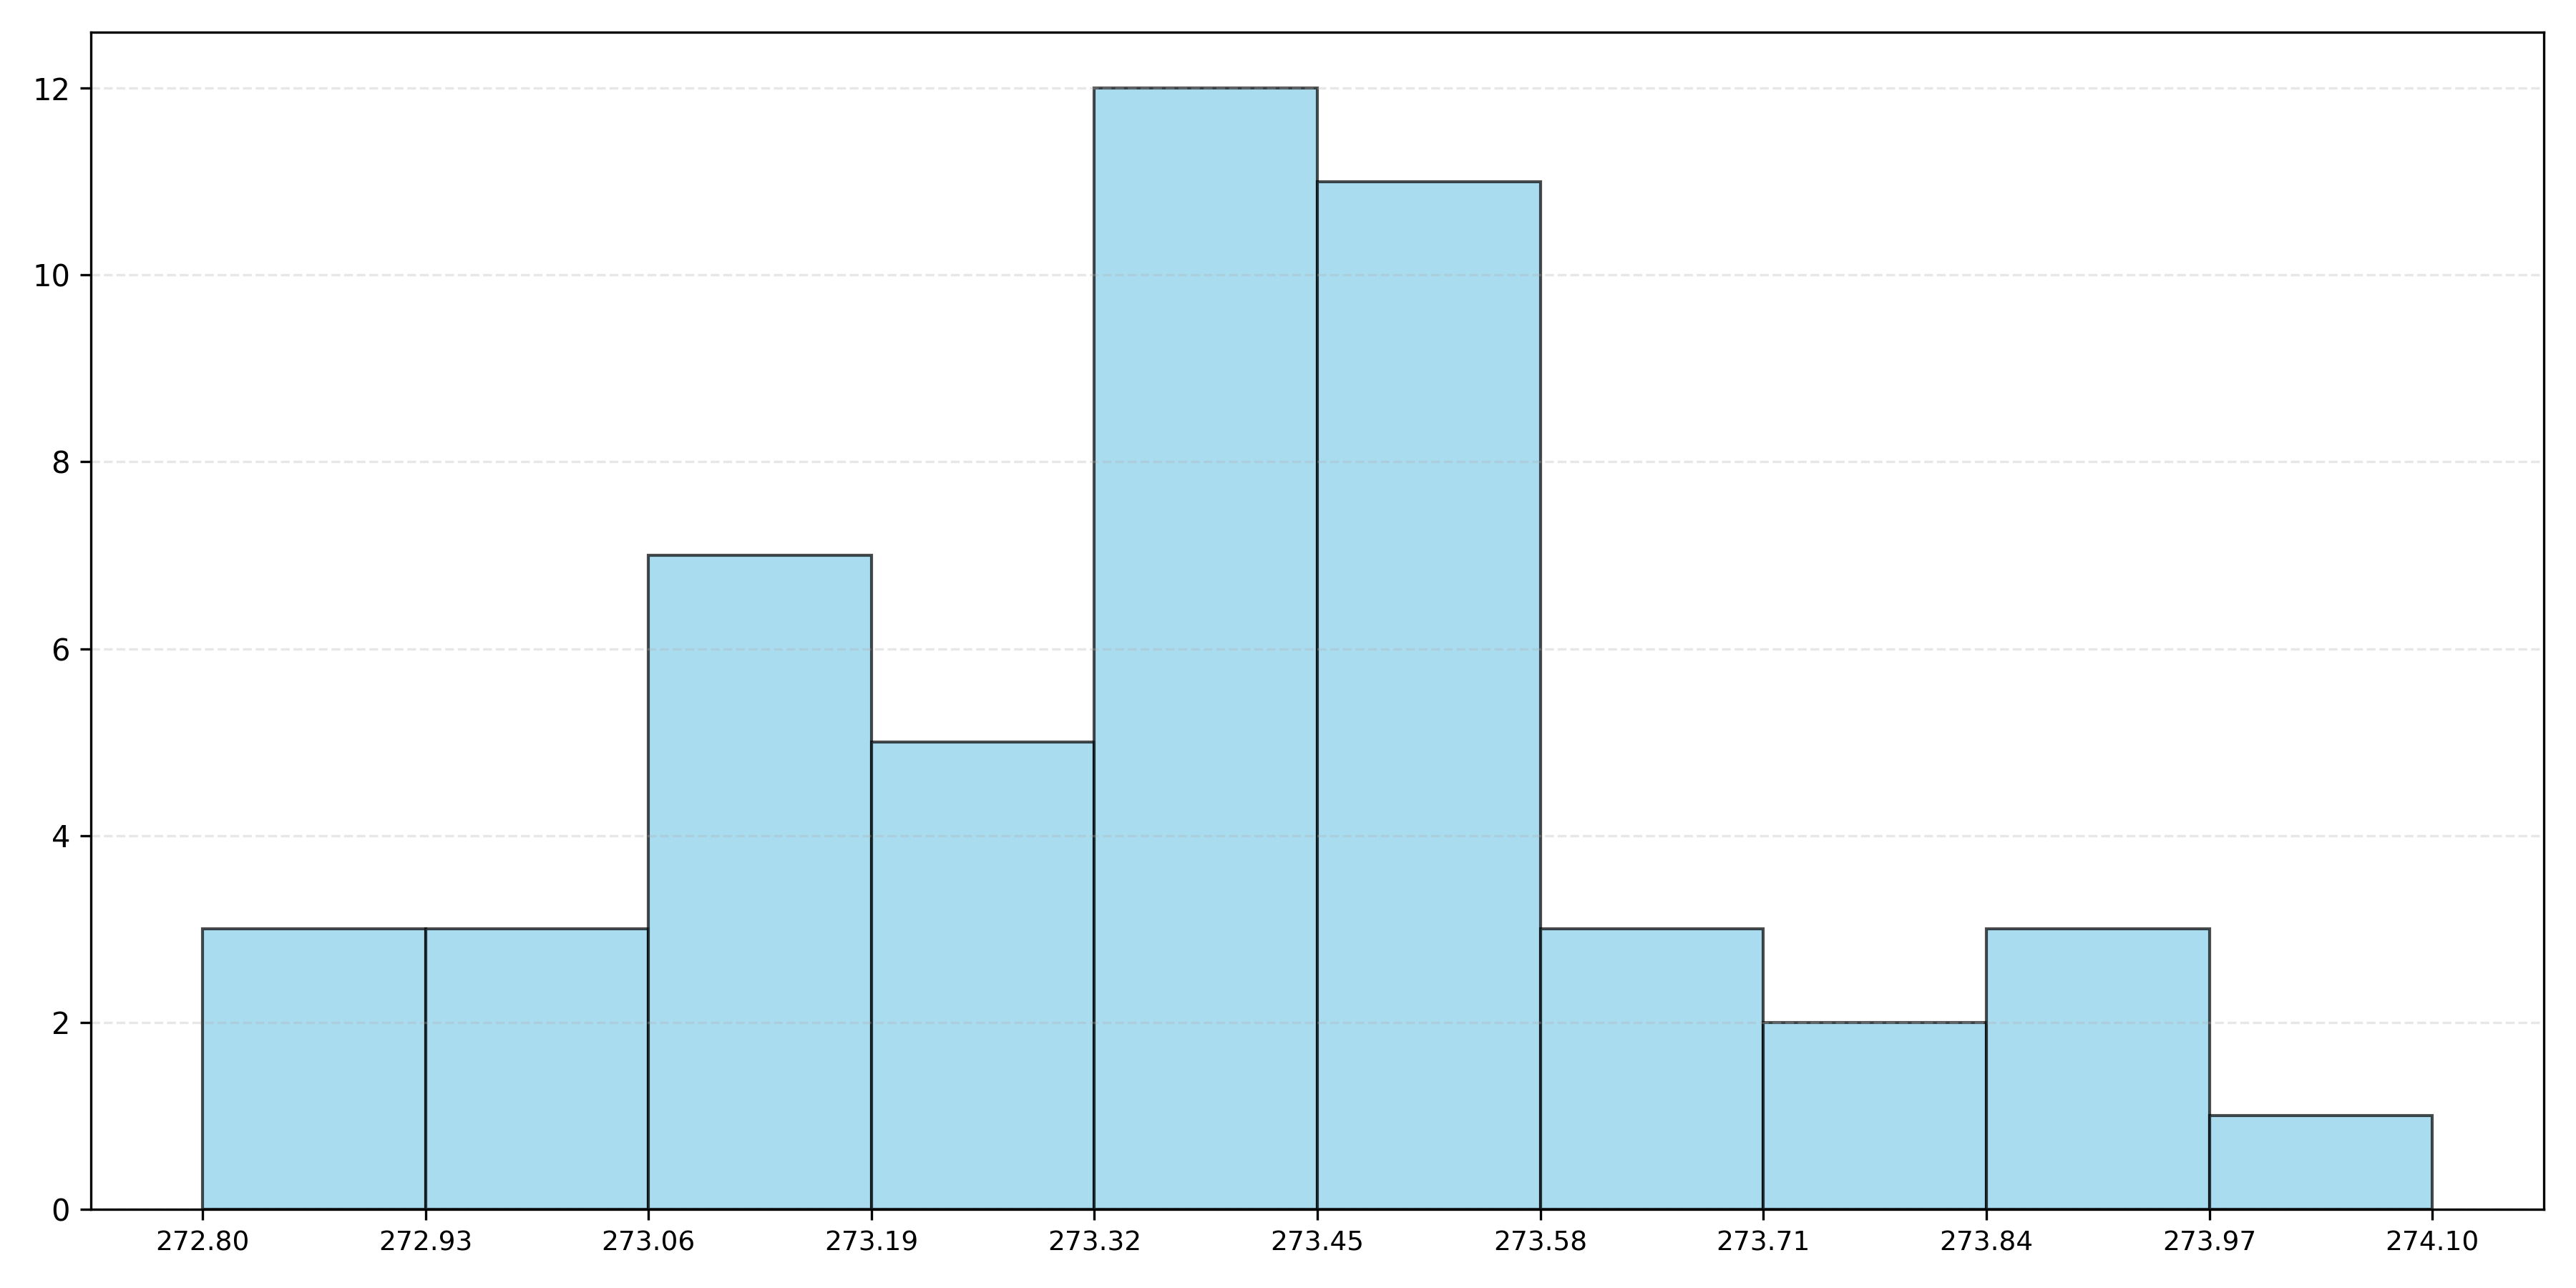
\includegraphics[width=0.8\textwidth]{histogram.png}
\caption{Гистограмма}
\end{figure}
И график плотности распределения
\begin{figure}[H]
\centering
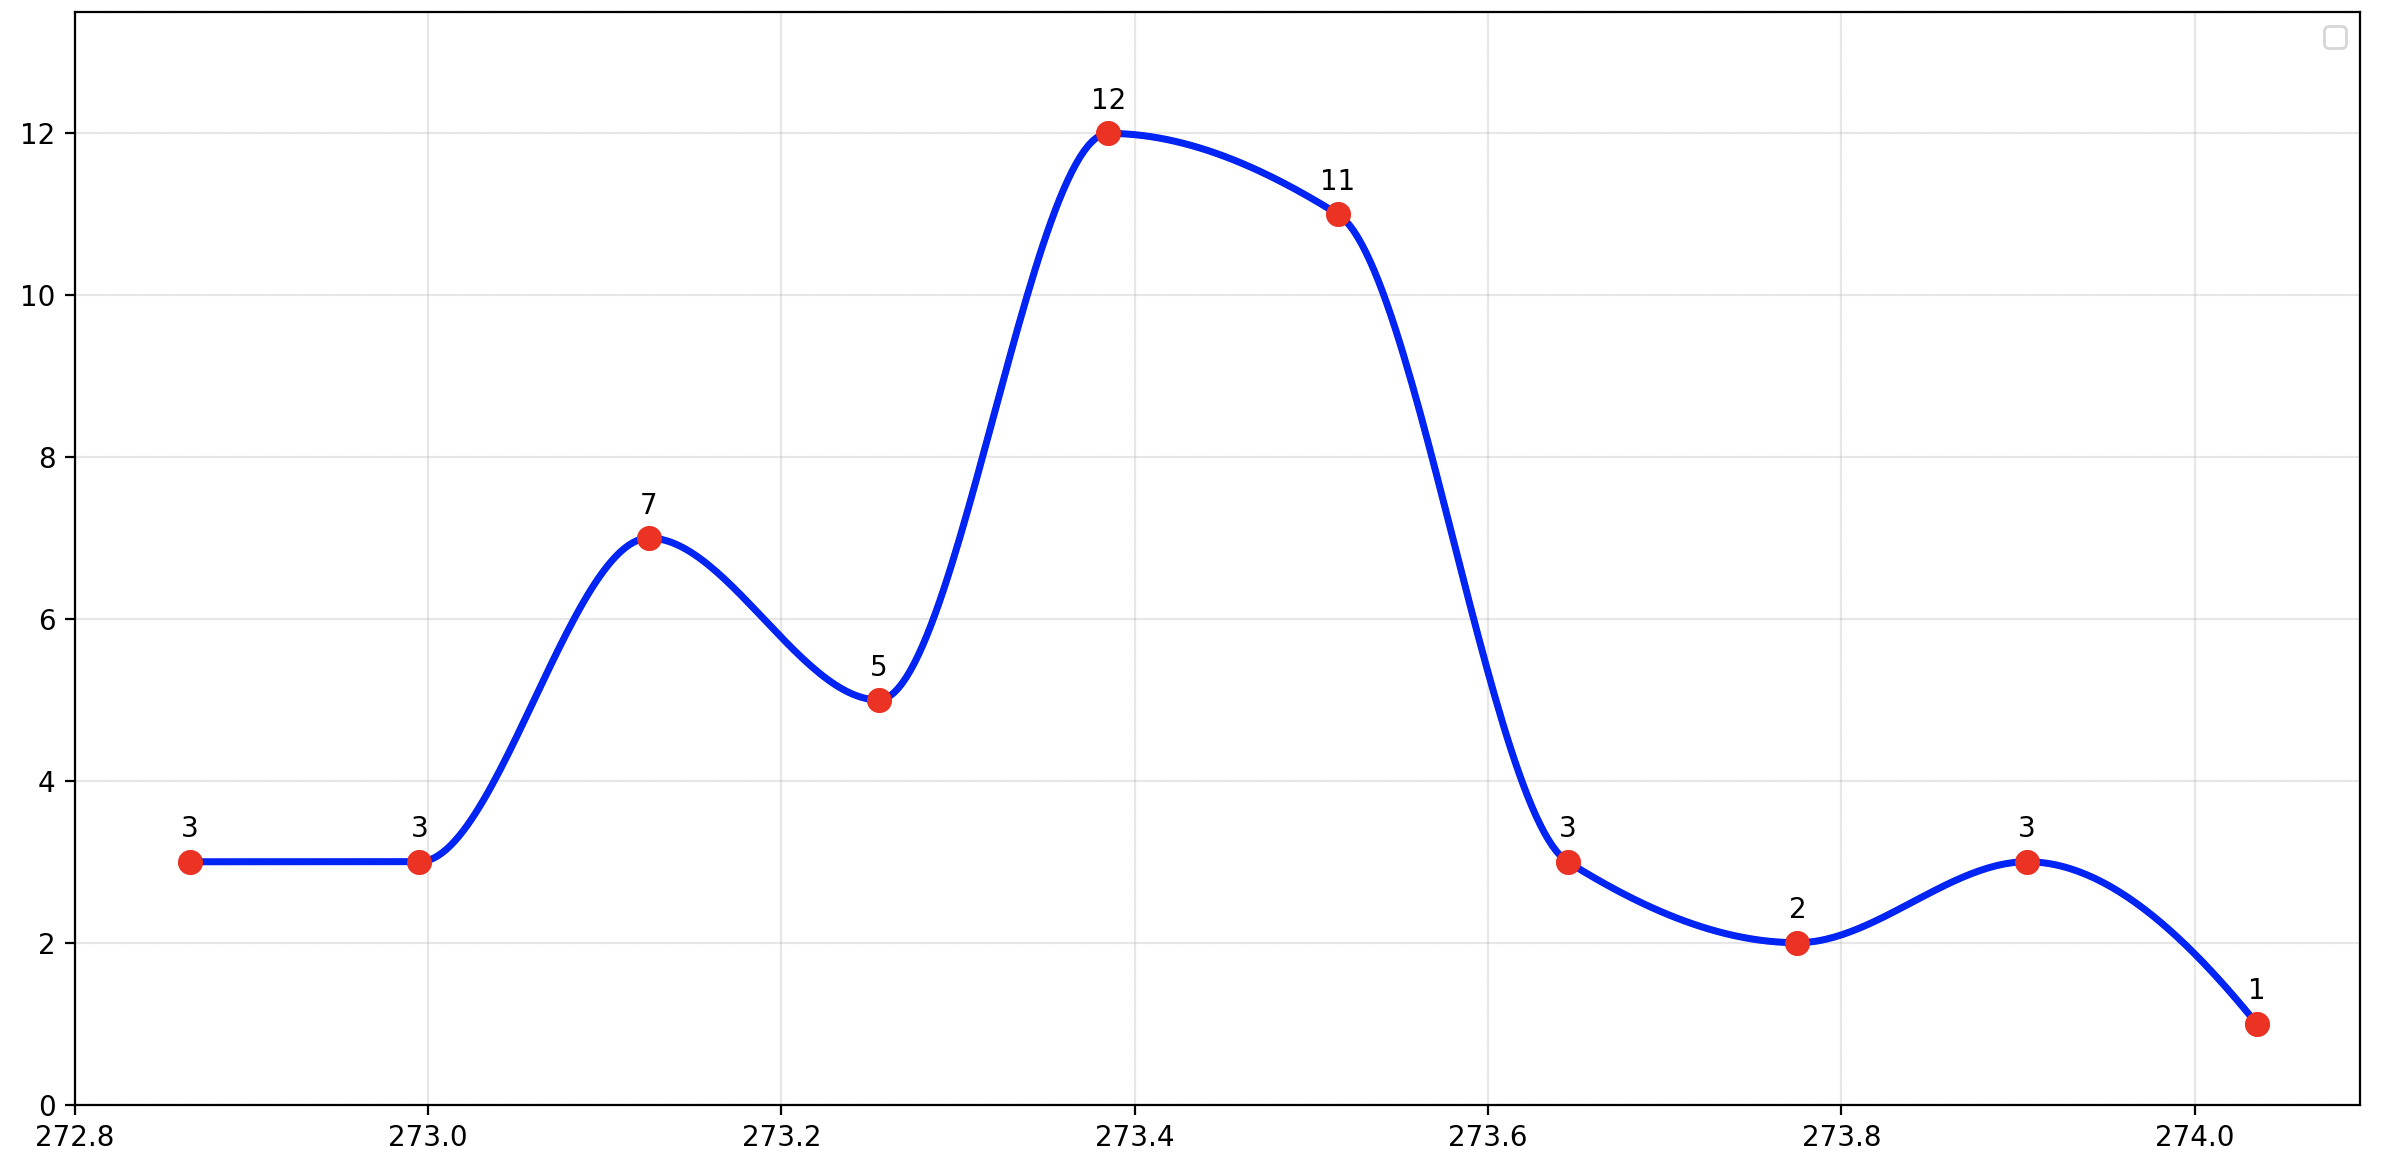
\includegraphics[width=0.8\textwidth]{dependency.png}
\caption{График зависимости}
\end{figure}
Для оценки разброса результатов рассчитывалось среднеквадратичное отклонение:

\begin{equation}
\sigma = \sqrt{\frac{1}{n-1}\sum_{i=1}^{n}(T_i - \overline{T})^2}.
\end{equation}

\begin{equation}
\sigma = 0,278
\end{equation}

На основании полученных данных вычислялась оценка средней квадратичной погрешности измерения

\begin{equation}
\sigma_{x} = \sigma/\sqrt{n}
\end{equation}

\begin{equation}
\sigma_{x} = 0,039
\end{equation}
и результат записывался в виде:

\[
T = \overline{T} \pm \Delta T.
\]
\begin{equation}
T = 273,389 \pm 0,039
\end{equation}

Для того чтобы оценить точность результатов, было проведено сравнение погрешности прибора $Delta T = 0,0011$ мс со случайной погрешностью $sigma_{x} = 0,039$. Поскольку случайная погрешность превышает приборную в 35 раз, сделан вывод о том что основной вклад вносит случайная погрешность.

\section{Выводы}

В ходе работы были проведены измерения электромеханических характеристик. Сравнение погрешности прибора со случайной погрешностью, показало, что приборная погрешность значительно меньше, что означает, что она не вносит основной вклад в погрешность измерений. 


\end{document}